\section{Dataset Construction} \label{sec:dataset-construction}

Recommender systems recommend items to users that are retrieved from some form of data storage. In the case of \emph{readnext}, this data storage takes the form of a dataset assembled from multiple sources.
This dataset will be referenced as \emph{base} or \emph{readnext} dataset throughout this thesis to distinguish it from the \emph{training}, \emph{validation}, and \emph{test} splits used for evaluation \Cref{sec:evaluation}.

Several factors must be considered during the construction of the \emph{readnext} dataset:

\begin{enumerate}
      \item The dataset must not be too \emph{small} as this would limit the number of potential recommendations, increasing the likelihood that none of the recommendations is relevant or that the user has already read many of the recommended papers.
            On the other hand, if the dataset is too \emph{large}, it could amplify the computational complexity of the recommender system and extend the waiting time for the user until recommendations are generated.
      \item The dataset must not be too \emph{narrow} in its coverage of research areas, as this would limit the number of users who could benefit from the recommender system.
            Conversely, the dataset must not be too \emph{broad}, as this would increase the likelihood that the recommendations are irrelevant to the user's research interests.
      \item The dataset should be reasonably \emph{up-to-date}. As the relevance of papers diminishes over time, the recommendations need to reflect the user's evolving research interests.
      \item All features requisite for the Hybrid Recommender must be present for each paper in the dataset. Documents with missing values that cannot be inferred from other observations, such as a missing paper abstract, are excluded from the dataset.
      \item The \emph{labels} for the evaluation must satisfy several conditions. First, they must be available for all papers in the dataset since they define which recommendations are considered relevant and which are deemed irrelevant.
            Second, they must be sufficiently granular to allow for a meaningful evaluation of the recommendations. For example, if the labeling scheme only covers two classes and each class is very broad, many recommended papers might be considered relevant even if they are only loosely related to the query paper.
            On the other hand, if the number of classes is too large and each class is highly specific, papers that are of high interest to the user might be considered irrelevant. Having excessively narrow classes can also prevent serendipitous and interdisciplinary recommendations, harming research diversity.
\end{enumerate}

\Cref{fig:dataset-construction} illustrates the different data sources for this thesis. The subsequent sections describe each data source in detail.

\begin{figure}[htb!]
      \centering
      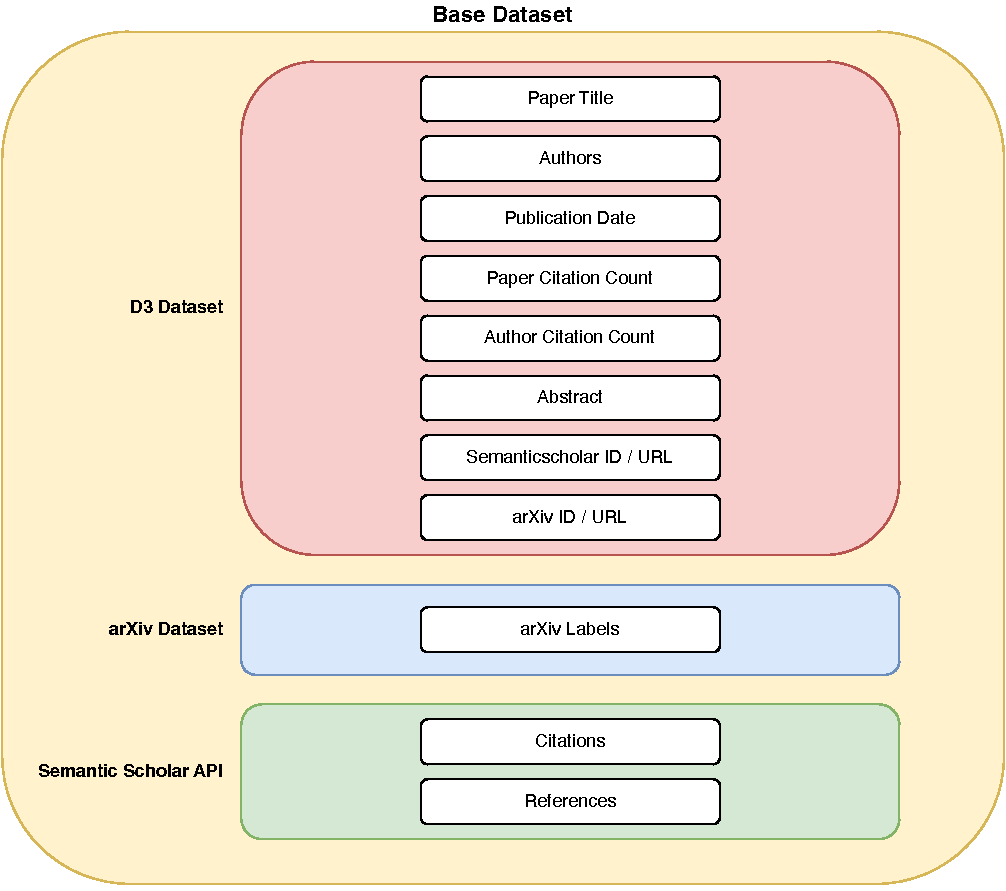
\includegraphics[width=0.9\textwidth]{diagrams/dataset_construction.pdf}
      \caption[Data Sources]{Data Sources used in this thesis. The D3 dataset provides paper metadata, including the publication date, citation counts and the paper abstract. ArXiv categories are added as evaluation labels from the arXiv Kaggle dataset. Lastly, the Semantic Scholar Academic Graph API is fetched to add lists of individual citations and references for each paper.}
      \label{fig:dataset-construction}
\end{figure}


\subsection{The D3 Dataset} \label{sec:d3-dataset}

The DBLP Discovery Dataset (D3) \cite{WahleD3Massive2022} is the primary data source for this thesis. Comprising over 6 million Computer Science papers, the D3 dataset is a curated compilation of research metadata harvested from the DBLP open-access repository\footnote{\url{https://dblp.org/}}. This metadata, which includes abstracts, author affiliations, and citation data, provides a comprehensive overview of the Computer Science research landscape.
Due to its high data quality, the D3 dataset has found application in multiple publications \cite{AbdallaElephantRoom2023,RuasCSInsightsSystem2023}.

Besides basic metadata such as titles, authors, and publication years provided by DBLP, the D3 dataset is further enriched with additional information that is parsed from PDF documents \cite{WahleD3Massive2022}.
As parsing PDF documents is notoriously prone to inaccuracies, the accuracy of the D3 dataset is not guaranteed.
Additionally, the D3 dataset only includes publications listed on DBLP, which might not encompass the complete spectrum of Computer Science research.

This thesis uses Version 2.1\footnote{\url{https://zenodo.org/record/7071698\#.ZA7jbC8w2Lc}} of the D3 dataset. Two files containing data about papers and authors can be downloaded in GZIP format from the Zenodo repository. Both datasets contain a unique author ID, which can be used to link the author information from the authors dataset to the paper information from the papers dataset.

The columns of both the "papers" and "authors" datasets are thoroughly documented on the D3 project's GitHub repository\footnote{\url{https://github.com/jpwahle/lrec22-d3-dataset}}. \emph{readnext} uses the following features from D3:

\begin{itemize}
      \item The \emph{paper title} and \emph{author names}. Although these variables are not directly used as features for the Hybrid Recommender, they are provided as additional context to the recommended papers.
      \item The \emph{publication date}, the \emph{paper citation count}, and the \emph{author citation counts}. These features are used as global document features for the Citation Recommender.
      \item The \emph{paper abstract}. This feature is used as input to the Language Recommender.
      \item The \emph{Semantic Scholar ID} and \emph{arXiv ID}.
            These features serve multiple purposes: First, they assist in merging labels (\Cref{sec:arxiv-labels}) as well as citation lists and reference lists (\Cref{sec:citation-features}) for each paper with the D3 dataset.
            Second, they are used as (external) unique identifiers for each paper. During the inference stage, they determine if the query paper from the user's input is already included in the \emph{readnext} corpus. Finally, the IDs are used to add the corresponding Semantic Scholar and arXiv URLs to the system's recommendations, facilitating immediate user access to the recommended papers.
\end{itemize}


\subsection{ArXiv Labels} \label{sec:arxiv-labels}

In order to determine whether the recommendations generated by the Hybrid Recommender are relevant or not, a ground-truth is required.
This ground-truth is obtained by using arXiv categories as labels. The primary reason for this choice is the mass availability in form of the arXiv Kaggle dataset\footnote{\url{https://www.kaggle.com/Cornell-University/arxiv}}, which contains data for over 1.7 million papers from the arXiv database.

The arXiv data is merged with the D3 dataset using the arXiv ID.
Since many papers in the D3 dataset do not possess a corresponding arXiv ID, this process results in a significant reduction of the dataset size.
Concretely, only $13,764$ papers out of the $100,000$ most cited papers in the D3 dataset have a corresponding arXiv ID.
The remaining papers lack essential label information needed for the \ac{MAP} computation during evaluation and are excluded from the dataset.

Unlike the \emph{ACM Computing Classification System}\footnote{\url{https://dl.acm.org/ccs}}, which contains narrow and nested categories, the arXiv categories are more coarse-grained with fewer and non-nested categories.
According to the \emph{arXiv category taxonomy}\footnote{\url{https://arxiv.org/category_taxonomy}}, there are $40$ categories within the Computer Science domain. Importantly, one paper is not restricted to a single category but can be assigned to multiple categories.
While arXiv distinguishes between primary and secondary classifications, the arXiv Kaggle dataset does not preserve this ordering. Thus, this thesis treats all categories equally.

One advantage of using arXiv categories as labels is that they are classified by the authors themselves.
This often results in precise category assignments, as authors, being experts in their research fields, typically classify their papers more accurately than automated systems.


\subsubsection*{Definition of Relevance}

The evaluation results crucially depend on the ground-truth definition for relevance.
For this thesis, we define a recommendation to be \emph{relevant} if the query paper and the recommended paper share at least one arXiv category. Conversely, it is classified as \emph{irrelevant} if the query paper and the recommended paper do not share any category.

To illustrate this definition with an example, consider the query paper \emph{Aspect-based Document Similarity for Research Papers} by Ostendorff et al. \cite{OstendorffAspectbasedDocument2020}, which is assigned the arXiv categories \emph{cs.CL} (Computation and Language) and \emph{cs.IR} (Information Retrieval).
Two candidate papers are considered, the first being \emph{BERT: Pre-training of Deep Bidirectional Transformers for Language Understanding} by Devlin et al. \cite{DevlinBERTPretraining2019}, which is assigned the arXiv label \emph{cs.CL} (Computation and Language). Since there is an overlap with the query labels, this recommendation is considered relevant. The second candidate paper is \emph{Deep Residual Learning for Image Recognition} by He et al. \cite{HeDeepResidual2015}, which is assigned the arXiv label \emph{cs.CV} (Computer Vision and Pattern Recognition). Since there is no overlap with the query labels, this recommendation is considered irrelevant.

The above definition is chosen over the alternative of classifying a recommendation relevant if query and recommended paper share \emph{all} categories for the following two reasons:
First, the number of papers that share all categories with the query paper is very small, leading to a highly unbalanced relevant/irrelevant ratio. Second, rewarding recommendations with at least one shared category allows for interdisciplinary recommendations since the query and candidate paper can still differ in multiple other categories.


\subsubsection*{Recommendation Diversity}

As highlighted in \Cref{sec:evaluation-of-recommender-systems}, non-accuracy-based metrics like diversity, serendipity, novelty, and coverage are often more difficult to quantify than their accuracy-based counterparts. However, these metrics provide essential insights into recommendation quality.
To capture some of these aspects, we propose a definition of \emph{recommendation diversity} that is specific to the context of this thesis.

Recommendation diversity is defined as the number of unique arXiv categories in the entire recommendation list. For example, if the recommendation list contains three papers with the arXiv categories \emph{cs.CL}, \emph{cs.IR}, and \emph{cs.CV}, the recommendation diversity is three. If the recommendation list contains three papers with the arXiv categories \emph{cs.CL}, \emph{cs.CL}, and \emph{cs.IR}, the recommendation diversity is two.
Since arXiv categories reflect research areas, recommendation diversity can be viewed as an indicator of interdisciplinarity within the recommendations.
As recommendations from different research areas are often unexpected, the recommendation diversity is closely related to serendipity.

This definition of diversity yields two insights. First, the diversity of a recommendation list is independent of the ranking order. Thus, the re-ranking process of the Hybrid Recommender does not affect the initial diversity of the candidate recommendations and it is sufficient to evaluate the diversity of the candidate lists generated by the Citation and Language Recommenders.

Second, there is not a perfect inverse correlation between a recommendation list's diversity and its \ac{MAP}, in which case the additional diversity metric would be redundant.
This observation arises because a single paper can belong to multiple research domains. For instance, recommendations for a query paper tagged with \emph{cs.CV} can display both high diversity and high \ac{MAP} if the suggested papers primarily come from the Computer Vision domain, complemented by papers from various other research areas.


\subsection{Citation Features} \label{sec:citation-features}

While the D3 dataset contains the number of cited and citing papers for each document, it does not contain lists of all \emph{individual} citations and references. As these are required to compute co-citation analysis and bibliographic coupling scores, an additional source is needed to supplement the dataset.
Therefore, data from the Semantic Scholar Academic Graph API\footnote{\url{https://api.semanticscholar.org/api-docs/graph}} is fetched.
To increase the rate limit, a private API key can be requested\footnote{\url{https://www.semanticscholar.org/product/api\#api-key}}.
The API allows for retrieving citation and reference lists for all papers in the dataset, which are subsequently added as new columns to the base dataset.

A significant limitation of the Semantic Scholar API is its restriction to request responses with a maximum of 1000 items. This leads to information loss for papers with more than 1000 citations or references.
Since only a single paper in the corpus cites more than $1000$ papers, namely \emph{A Survey of Neuromorphic Computing and Neural Networks in Hardware} by Schuman et al. \cite{SchumanSurveyNeuromorphic2017}, the bibliographic coupling scores are barely affected by this limitation.
However, the co-citation analysis scores are heavily affected since $868$ papers are cited more than $1000$ times.
These frequently cited papers are thus represented with a too weak connection to the related literature.

While this constraint may introduce bias in the dataset, the paper citation count feature of the Citation Recommender might offset its impact.
Larger weights can be assigned to paper citation counts for highly cited papers to counteract the truncated co-citation analysis scores.
